\subsection{The room size enumeration type}
\label{sec:application:building_the_model:the_room_size_enumeration_type}

In the sixth step, a new type will be introduced. This time around, it will not be a class type, but an enumeration type. It is the $.\type{RoomSize}$ enumeration type used to specify the room sizes. \cref{subsec:library_of_transformations:type_level_transformations:enumeration_types} is used to introduce the enumeration type on the type level, while on the instance level, \cref{subsec:library_of_transformations:instance_level_transformations:enumeration_values} is used to introduce the values of the enumeration.

The $name$ of the new enumeration type is $.\type{RoomSize}$, and it has $values = \{\type{SMALL}, \type{MEDIUM}, \type{LARGE}\}$. Please note that there are multiple encodings possible to encode an enumeration type in GROOVE. The encoding using flags is chosen for this enumeration type. The function $fob$ which maps the enumeration values to internal node ids is defined as follows:
\begin{align*}
    fob = \{&(\type{SMALL}, \text{SmallSize}), (\type{MEDIUM}, MediumSize), (\type{LARGE}, LargeSize)\}
\end{align*}

The function $fid$ which maps the enumeration values to explicit node identifiers is equal to the definition of $fob$, so $fid = fob$. The following model is obtained:

\LTXtable{\textwidth}{tex/06_application/02_building_the_model/tables/06_the_room_size_enumeration_type.tex}

\begin{figure}[p]
    \centering
    \begin{subfigure}{0.98\textwidth}
        \centering
        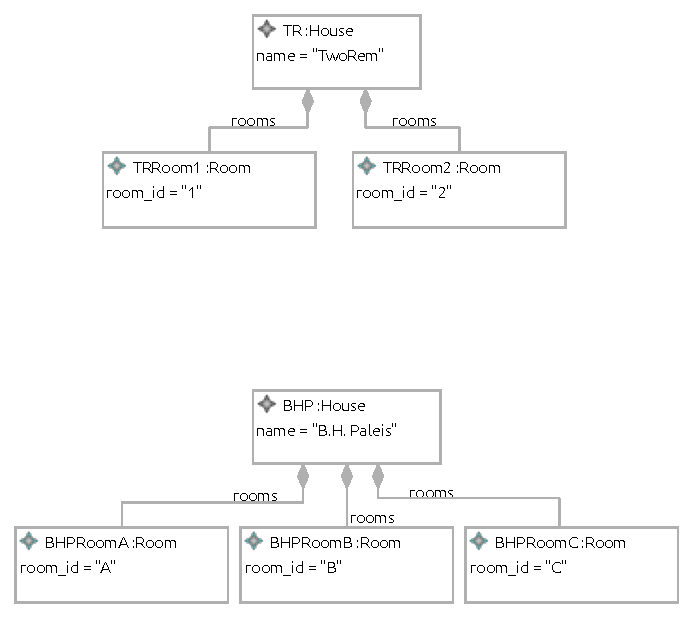
\includegraphics{images/06_application/instance_model/step06.pdf}
        \caption{Instance Model $Im_6$}
        \label{fig:application:building_the_model:the_room_size_enumeration_type:ecore:instance_model}
    \end{subfigure}
    \\
    \begin{subfigure}{0.98\textwidth}
        \centering
        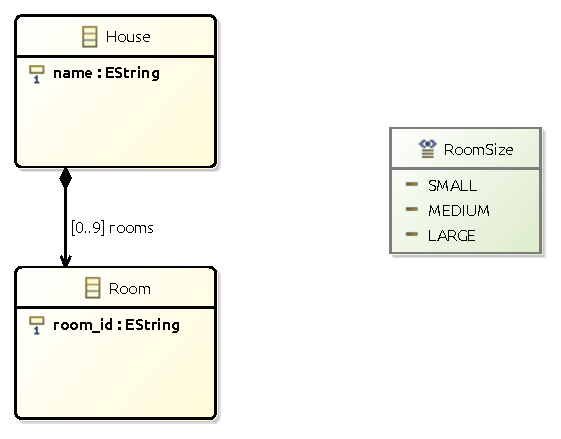
\includegraphics{images/06_application/type_model/step06.pdf}
        \caption{Type Model $Tm_6$}
        \label{fig:application:building_the_model:the_room_size_enumeration_type:ecore:type_model}
    \end{subfigure}
    \caption{The Ecore model after step 6}
    \label{fig:application:building_the_model:the_room_size_enumeration_type:ecore}
\end{figure}

\begin{figure}[p]
    \centering
    \begin{subfigure}{0.98\textwidth}
        \centering
        % To use this figure in your LaTeX document
% import the package groove/resources/groove2tikz.sty
%
\begin{tikzpicture}[scale=\tikzscale,name prefix=step06-]
\node[basic_node] (n0) at (2.740, -4.200) {\ml{\uline{\textit{BHP}} : \textbf{House}\\name = "B.H. Paleis"}};
\node[basic_node] (n1) at (2.660, -0.340) {\ml{\uline{\textit{TR}} : \textbf{House}\\name = "TwoRem"}};
\node[basic_node] (n4) at (2.760, -2.060) {\ml{\uline{\textit{SmallSize}} : \textbf{RoomSize}\\\textit{SMALL}}};
\node[basic_node] (n5) at (4.410, -0.570) {\ml{\uline{\textit{MediumSize}} : \textbf{RoomSize}\\\textit{MEDIUM}}};
\node[basic_node] (n6) at (0.990, -0.550) {\ml{\uline{\textit{LargeSize}} : \textbf{RoomSize}\\\textit{LARGE}}};
\node[basic_node] (n7) at (1.820, -1.470) {\ml{\uline{\textit{TRRoom1}} : \textbf{Room}\\room\_id = "1"}};
\node[basic_node] (n8) at (3.410, -1.480) {\ml{\uline{\textit{TRRoom2}} : \textbf{Room}\\room\_id = "2"}};
\node[basic_node] (n14) at (0.820, -3.060) {\ml{\uline{\textit{BHPRoomA}} : \textbf{Room}\\room\_id = "A"}};
\node[basic_node] (n15) at (2.780, -3.050) {\ml{\uline{\textit{BHPRoomB}} : \textbf{Room}\\room\_id = "B"}};
\node[basic_node] (n16) at (4.720, -3.060) {\ml{\uline{\textit{BHPRoomC}} : \textbf{Room}\\room\_id = "C"}};

\path[basic_edge] (n0)  --  (n14) 
node[lab] at (1.584, -3.455) {\ml{rooms}};
\path[basic_edge](n0.north -| 2.780, -3.050) -- node[lab] {\ml{rooms}} (n15) ;
\path[basic_edge] (n0)  -- node[lab] {\ml{rooms}} (n16) ;
\path[basic_edge] (n1)  -- node[lab] {\ml{rooms}} (n7) ;
\path[basic_edge] (n1)  -- node[lab] {\ml{rooms}} (n8) ;
\end{tikzpicture}

        \caption{Instance Graph $IG_6$}
        \label{fig:application:building_the_model:the_room_size_enumeration_type:groove:instance_graph}
    \end{subfigure}
    \\
    \begin{subfigure}{0.98\textwidth}
        \centering
        % To use this figure in your LaTeX document
% import the package groove/resources/groove2tikz.sty
%
\begin{tikzpicture}[scale=\tikzscale,name prefix=step06-]
\node[basic_node] (n0) at (2.740, -4.200) {\ml{\uline{\textit{BHP}} : \textbf{House}\\name = "B.H. Paleis"}};
\node[basic_node] (n1) at (2.660, -0.340) {\ml{\uline{\textit{TR}} : \textbf{House}\\name = "TwoRem"}};
\node[basic_node] (n4) at (2.760, -2.060) {\ml{\uline{\textit{SmallSize}} : \textbf{RoomSize}\\\textit{SMALL}}};
\node[basic_node] (n5) at (4.410, -0.570) {\ml{\uline{\textit{MediumSize}} : \textbf{RoomSize}\\\textit{MEDIUM}}};
\node[basic_node] (n6) at (0.990, -0.550) {\ml{\uline{\textit{LargeSize}} : \textbf{RoomSize}\\\textit{LARGE}}};
\node[basic_node] (n7) at (1.820, -1.470) {\ml{\uline{\textit{TRRoom1}} : \textbf{Room}\\room\_id = "1"}};
\node[basic_node] (n8) at (3.410, -1.480) {\ml{\uline{\textit{TRRoom2}} : \textbf{Room}\\room\_id = "2"}};
\node[basic_node] (n14) at (0.820, -3.060) {\ml{\uline{\textit{BHPRoomA}} : \textbf{Room}\\room\_id = "A"}};
\node[basic_node] (n15) at (2.780, -3.050) {\ml{\uline{\textit{BHPRoomB}} : \textbf{Room}\\room\_id = "B"}};
\node[basic_node] (n16) at (4.720, -3.060) {\ml{\uline{\textit{BHPRoomC}} : \textbf{Room}\\room\_id = "C"}};

\path[basic_edge] (n0)  --  (n14) 
node[lab] at (1.584, -3.455) {\ml{rooms}};
\path[basic_edge](n0.north -| 2.780, -3.050) -- node[lab] {\ml{rooms}} (n15) ;
\path[basic_edge] (n0)  -- node[lab] {\ml{rooms}} (n16) ;
\path[basic_edge] (n1)  -- node[lab] {\ml{rooms}} (n7) ;
\path[basic_edge] (n1)  -- node[lab] {\ml{rooms}} (n8) ;
\end{tikzpicture}

        \caption{Type Graph $TG_6$}
        \label{fig:application:building_the_model:the_room_size_enumeration_type:groove:type_graph}
    \end{subfigure}
    \caption{The GROOVE graphs after step 6}
    \label{fig:application:building_the_model:the_room_size_enumeration_type:groove}
\end{figure}

A visual representation of $Tm_6$ and $Im_6$ can be found in \cref{fig:application:building_the_model:the_room_size_enumeration_type:ecore}. Similarly, a visual representation of $TG_6$ and $IG_6$ can be found in \cref{fig:application:building_the_model:the_room_size_enumeration_type:groove}. Please note that because of the definitions of $f_6(Im_6)$ and $f'_6(IG_6)$, we have that $f_6(Im_6) = IG_6$ and $f'_6(IG_6) = Im_6$. Furthermore, $f_6(Im_6)$ and $f'_6(IG_6)$ are valid mapping functions themselves, such that they can be combined with another mapping function in the next step.

The introduction of the enumeration type shows the encoding of an enumeration type as GROOVE flags in practice. It should be noted that although the instance model has not changed, the instance graph obtained instances of the enumeration values. These instances will be referenced by an enumeration field in the next step.

\afterpage{\FloatBarrier}